% ****** Start of file apssamp.tex ******
%
%   This file is part of the APS files in the REVTeX 4.1 distribution.
%   Version 4.1r of REVTeX, August 2010
%
%   Copyright (c) 2009, 2010 The American Physical Society.
%
%   See the REVTeX 4 README file for restrictions and more information.
%
% TeX'ing this file requires that you have AMS-LaTeX 2.0 installed
% as well as the rest of the prerequisites for REVTeX 4.1
%
% See the REVTeX 4 README file
% It also requires running BibTeX. The commands are as follows:
%
%  1)  latex apssamp.tex
%  2)  bibtex apssamp
%  3)  latex apssamp.tex
%  4)  latex apssamp.tex
%
\documentclass[%
 reprint,
%superscriptaddress,
%groupedaddress,
%unsortedaddress,
%runinaddress,
%frontmatterverbose,
%preprint,
%showpacs,preprintnumbers,
%nofootinbib,
%nobibnotes,
%bibnotes,
 amsmath,amssymb,
 aps,
%pra,
%prb,
%rmp,
%prstab,
%prstper,
%floatfix,
]{revtex4-1}

\usepackage{graphicx}% Include figure files
\usepackage{dcolumn}% Align table columns on decimal point
\usepackage{bm}% bold math
\usepackage{algorithm}
\usepackage{algorithmicx}
\usepackage{algpseudocode}
\usepackage{color}
%\usepackage{hyperref}% add hypertext capabilities
%\usepackage[mathlines]{lineno}% Enable numbering of text and display math
%\linenumbers\relax % Commence numbering lines

%\usepackage[showframe,%Uncomment any one of the following lines to test
%%scale=0.7, marginratio={1:1, 2:3}, ignoreall,% default settings
%%text={7in,10in},centering,
%%margin=1.5in,
%%total={6.5in,8.75in}, top=1.2in, left=0.9in, includefoot,
%%height=10in,a5paper,hmargin={3cm,0.8in},
%]{geometry}

\begin{document}

\preprint{APS/123-QED}

\title{The {\it ab initio\/} calculation of molecular properties as quasi-energy derivatives}% Force line breaks with \\
%\thanks{A footnote to the article title}%

\author{Kenneth Ruud}
 \affiliation{Hylleraas Centre for Quantum Molecular Sciences, Department of Chemistry, UiT The Arctic University of Norway, 9037 Troms\o , Norway}%Lines break automatically or can be forced with \\
\author{Magnus Ringholm}%
% \email{Second.Author@institution.edu}
\affiliation{%
 Authors' institution and/or address}%

\author{Radovan Bast}
% \homepage{http://www.Second.institution.edu/~Charlie.Author}
\affiliation{Department of Computer Services, UiT The Arctic University of Norway, 9037 Tromsø, Norway% with \\
}%
\author{Simen Reine}
\affiliation{%
 Hylleraas Centre for Quantum Molecular Sciences, Department of Chemistry, University of Oslo, P.O.Box 1033 Blindern, 0315 Oslo, Norway}
%

\date{\today}% It is always \today, today,
             %  but any date may be explicitly specified


\def\im{\mathrm{i}}
\def\ket#1{|#1\rangle}
\def\bra#1{\langle#1|}
\def\brau#1{\langle#1}
\def\bfr{{\bf r}}
\def\bfx{{\bf x}}
\def\bfX{{\bf X}}
\def\bfS{{\bf S}}
\def\bfD{{\bf D}}
\def\bfG{{\bf G}}
\def\bfc{{\bf c}}
\def\barx{{\bf \bar x}}
\def\barD{{\bf \bar D}}
\def\tildeD{{\bf \tilde D}}
\def\bfEone#1{{\bf E_{#1}^{(1)}}}
\def\bfF#1{{\bf F_{#1}}}
\def\bfeone{{\bf e^{(1)}}}
\def\bfEtwo#1{{\bf E_{#1}^{(2)}}}
\def\bfetwo{{\bf e^{(2)}}}
\def\bfkappa{{\boldsymbol \kappa}}
\def\bfs{\boldsymbol}
\def\Kappa{{K}}
\def\sgn{\text{sgn}}
\def\vec{\text{vec}}
\def\tildex{{\bf \tilde x}}
\def\expectation#1#2{\langle#1|#2\rangle}
\def\Tr{\mbox{Tr}}
\def\bfL{{\boldsymbol \Gamma}}
\def\Ld{\Gamma^{\dagger}}
\def\bm#1{\mbox{\boldmath $ #1 $}}
% Macro for expectation value <0|[#1,#2]0>
\def\expc#1#2{\bra{0}[#1,#2]\ket{0}}
% Macro for expectation value <0|[[#1,#2],#3]0>
\def\expcc#1#2#3{\bra{0}[[#1,#2],#3]\ket{0}}
% Macro for expectation value <0|[#1,[#2,#3]]0>
\def\expccr#1#2#3{\bra{0}[#1,[#2,#3]]\ket{0}}
% Macro for expectation value <0|[[[#1,#2],#3],#4]0>
\def\expccc#1#2#3#4{\bra{0}[[[#1,#2],#3],#4]\ket{0}}
% Macro for expectation value <0|[[[#1,#2],#3],#4]0>
\def\expcccr#1#2#3#4{\bra{0}[#1,[#2,[#3,#4]]]\ket{0}}

\newcommand{\fixme}[1]{{\small\em \color{red} \marginpar{\mbox{$\Longleftarrow$}} #1 \normalsize}}


\begin{abstract}
An article usually includes an abstract, a concise summary of the work
covered at length in the main body of the article.
%\begin{description}
%\item[Usage]
%Secondary publications and information retrieval purposes.
%\item[PACS numbers]
%May be entered using the \verb+\pacs{#1}+ command.
%\item[Structure]
%You may use the \texttt{description} environment to %structure your abstract;
%use the optional argument of the \verb+\item+ command to %give the category of each item.
%\end{description}
\end{abstract}

%\pacs{Valid PACS appear here}% PACS, the Physics and Astronomy
                             % Classification Scheme.
%\keywords{Suggested keywords}%Use showkeys class option if keyword
                              %display desired
\maketitle

%\tableofcontents

\section{\label{sec:intro}Introduction}



\section{\label{sec:MolProp}Molecular Properties as energy derivatives}

\subsection{Variational perturbation theory}

The calculation of molecular properties using the flexible tools of response
theory~\cite{} is often hampered by the lengthy equations that follows from the
formalism when expanding the energy in orders of the applied perturbation. This
is also the case when we consider derivatives of the quasi-energy~\cite{}, as
we will see in Section~\ref{rsp_theory}. Nevertheless, the underlying
principles are rather simple, the complications often arising from the explicit
parametrization of the wave function theory used. Variational perturbation
theory provides a simple framework to illustrate these principles, and will
also provide us with a nice framework to link energy-derivative theory to
perturbation theory.

Let us consider an electronic energy $E\equiv
E\left(\lambda,\varepsilon\right)$ that depends on a set of variational
parameters $\lambda$ describing the wave function used to study the molecular
system as well as some perturbations collected in a vector $\varepsilon$. The
variational parameters will in the case of Hartree--Fock and Kohn--Sham
density-functional theory~(KS-DFT) be the molecular orbital coefficients. In
the case of multiconfigurational self-consistent field wave functions~(MCSCF),
the variational parameters will include the weights of the different excited
Slater determinants defined by the chosen active orbitals, in addition to the
MO coefficients. The fact that the wave function will change when a
perturbation $\varepsilon$ is applied, such as an external electric field $F$,
implies that the variation parameters have an implicit dependence on the
applied perturbations, $\lambda\equiv \lambda\left(\varepsilon\right)$. This
means that when we apply a perturbation, the change in the energy will have two
contributions, one from the explicity dependence of the Hamiltonian on the
perturbation, and one from the implicit dependence of the variational
parameters on the perturbation

\begin{equation}
\frac{dE}{d\varepsilon_a} = \frac{\partial E}{\partial\varepsilon_a} + \sum_i
\frac{\partial
  E}{\partial\lambda_i}\frac{\partial\lambda_i}{\partial\varepsilon_a}.
\label{eq:variation}
\end{equation}

The choice of HF, KS-DFT or MCSCF above as examples was deliberate, as these
methods are all methods that are considered to be {\em variational\/} methods,
that is, the energy is stationary with respect to all variational parameters
and that this can be enforced for any strength of an applied perturbation

\begin{equation}
\frac{dE}{d\lambda_i} = \frac{\partial E}{\partial\lambda_i} =
0\qquad\forall i, \varepsilon
\label{eq:varcondition}
\end{equation}
where the equivalence of the absolute and partial derivatives arise because
$\lambda$ and $\varepsilon$ are independent variables. Inserting
Eq.~\eqref{eq:varcondition} into Eq.~\eqref{eq:variation}, we get

\begin{equation}
\frac{dE}{d\varepsilon_a} = \frac{\partial E}{\partial\varepsilon_a},
\end{equation}
that is, the first-order variation in the energy is determined by the
dependence of the Hamiltonian on the perturbation since
$E=\langle\Psi\mid\hat{H}\mid\Psi\rangle$, and thus is given as the expectation
value

\begin{equation}
\frac{dE}{d\varepsilon_a} = \langle\Psi\mid\frac{\partial
  \hat{H}}{\partial \varepsilon_a}\mid\Psi\rangle
\end{equation}
which is the well-known Hellmann-Feynman theorem. We emphasize that {\em
variational\/} should not be confused with wave functions determined from the
application of the variational principle. Configuration Interaction~(CI) wave
functions are for instance determined by applying the variational principle,
but as it is only applied to the CI coefficients, and not the MO coefficients,
the CI wave functions does not satisfy Eq.~\eqref{eq:varcondition}. For such
{\em non-variational} wave functions, the Hellmann-Feynmann theorem will not
give the same result as the energy variation given in Eq.~\eqref{eq:variation}.
We note in passing that through the use of Langrange multipliers,
non-variational wave functions can be cast in a variational
form.~\cite{HelgakerJorgensen,PRSBook}

Before considering second-order variations in the energy to external
perturbations, let us first consider how the variational condition
Eq.~\eqref{eq:varcondition} depends on an external perturbation.
Differentiating Eq.~\eqref{eq:varcondition} with respect to a perturbation
$\varepsilon_a$, we get

\begin{equation}
\frac{d^2E}{d\lambda_id\varepsilon_a} =
\frac{\partial^2E}{\partial\lambda_i\partial\varepsilon_a} +
\sum_j\frac{\partial^2E}{\partial\lambda_i\partial\lambda_j}\frac{\partial\lambda_j}{\partial\varepsilon_a}
= 0.\label{eq:1ordervar}
\end{equation}
where the last equality comes from differentiating the right-hand side of
Eq.~\eqref{eq:varcondition}. We can rewrite Eq.~\eqref{eq:1ordervar} to give us
an expression for the first-order variation of the variational parameters with
respect to the external perturbation

\begin{equation}
\frac{\partial\lambda_j}{\partial\varepsilon_a} =
-\sum_i\left(\frac{\partial^2E}{\partial\lambda_i\partial\lambda_j}\right)^{-1}\frac{\partial^2E}{\partial\lambda_i\partial\varepsilon_a}.
\end{equation}
Let us now proceed to second-order variations in the energy. Differentiating
Eq.~\eqref{eq:variation} with respect to a second perturbation, we get

\begin{align}
  \frac{d^2E}{d\varepsilon_a d\varepsilon_b} &= \frac{\partial^2
    E}{\partial\varepsilon_a\partial\varepsilon_b} +
  \sum_i\frac{\partial^2E}{\partial\varepsilon_a\partial\lambda_i}\frac{\partial\lambda_i}{\partial\varepsilon_b}
  +
  \sum_i\frac{\partial^2E}{\partial\varepsilon_b\partial\lambda_i}\frac{\partial\lambda_i}{\partial\varepsilon_a}\nonumber\\
  &+
  \sum_{i,j}\frac{\partial^2E}{\partial\lambda_i\partial\lambda_j}\frac{\partial\lambda_i}{\partial\varepsilon_a}\frac{\partial\lambda_j}{\partial\varepsilon_b}
  + \sum_i\frac{\partial
    E}{\partial\lambda_i}\frac{\partial^2\lambda_i}{\partial\varepsilon_a\partial\varepsilon_b}\label{eq:Full2ndorder}
\end{align}
Using Eqs.~\eqref{eq:varcondition} and~\eqref{eq:1ordervar}, we can rewrite the
expression for the second-order variation in several different equivalent forms

\begin{align}
\frac{d^2E}{d\varepsilon_a d\varepsilon_b} &= \frac{\partial^2
    E}{\partial\varepsilon_a\partial\varepsilon_b} +
\sum_i\frac{\partial^2E}{\partial\varepsilon_a\partial\lambda_i}\frac{\partial\lambda_i}{\partial\varepsilon_b}\nonumber\\
 &= \frac{\partial^2
  E}{\partial\varepsilon_a\partial\varepsilon_b} +
\sum_i\frac{\partial^2E}{\partial\varepsilon_b\partial\lambda_i}\frac{\partial\lambda_i}{\partial\varepsilon_a}\label{eq:2ndorder}\\
 &= \frac{\partial^2
  E}{\partial\varepsilon_a\partial\varepsilon_b} -
\sum_{i,j}\frac{\partial^2
  E}{\partial\varepsilon_a\partial\lambda_i}\left(\frac{\partial^2
E}{\partial\lambda_i\partial\lambda_j}\right)^{-1}\frac{\partial^2
  E}{\partial\varepsilon_b\partial\lambda_j}\nonumber
\end{align}
Eq.~\eqref{eq:2ndorder} is somewhat pedantic, but together with
Eq.~\eqref{Full2ndorder} it illustrates a number of important principles used
in the evaluation of molecular response properties.

First of all, Eq.~\eqref{eq:2ndorder} shows that we can calculate second-order
corrections to the energy from a knowledge of the first-order variations in the
wave function parameters only. This is again due to the variational condition,
Eq.~\eqref{eq:varcondition}. This, as well as the Hellmann--Feynman theorem,
are more general examples of what is referred to as the $2n+1$ rule of energy
derivative theory: Knowing the perturbed wave function to order $n$, allows you
to calculate energy corrections to order $2n+1$, often referred to as the
Wigner $2n+1$ rule.~\cite{Hylleraas1930,Wigner1930} There exist different rules
for order of perturbed variational parameters, and we will return briefly to
this in Section~\ref{rsp_theory}.

The two first lines of Eq.~\eqref{eq:2ndorder} also illustrates a second
important principles, namely that we can generate the perturbed wave-function
parameters from either of the two applied perturbations, $\varepsilon_a$ or
$\varepsilon_b$. This is often referred to as the interchange
theorem~\cite{Interchange} and allows you to determine the perturbed wave
function for the perturbations with the fewest components. This is important
computationally, as the most time-consuming step of a molecular property
calculation is the determination of the perturbed wave function.

As an example of how this can be utilized, consider the nuclear magnetic
shielding constants determined in nuclear magnetic resonance spectroscopy
(NMR).~\cite{ChemRev1999,ChemRev2012} These shielding constants are the mixed
second-order derivatives of the molecular energy with respect to an external
magnetic field and the nuclear magnetic moments. Whereas there are only three
components of the magnetic field, there are three components of the magnetic
moment of each atom in the molecule with a nuclear spin. Only the perturbed
variational parameters for the the external magnetic field components thus need
to be determined, and the cost of calculating of shielding constants are thus
largely independent of molecular size. The $2n+1$ rule and the interchange
theorem has also been used with advantage to calculate all spin--spin coupling
constants in C$_{60}$ in an efficient manner~\cite{JaszunskiC60} or to enable
linear-scaling calculations of NMR shielding constants in large molecular
systems.~\cite{Ochsenfeld}

The last equality in Eq.~\eqref{eq:2ndorder} is not particularly important from
a computationally point of view, as it would involve determining the perturbed
variational parameters for all applied perturbations. However, it is a bridge
to link energy-derivative theory to perturbation theory.

We will not pursue these derivations any further, but just to illustrate the
$2n+1$ rule, we here give the expression for the third-order energy correction
using only first-order perturbed wave function parameters

\begin{align}
\label{eq:erg3}
\frac{d^{3}E}{d\varepsilon_ad\varepsilon_bd\varepsilon_c}
 & =
\frac{\partial^{3}E}{\partial\varepsilon_a\partial\varepsilon_b\partial\varepsilon_c}+\frac{\partial^{3}E}{\partial\varepsilon_a\partial\varepsilon_b\partial\lambda_{i}}\frac{\partial\lambda_{i}}{\partial\varepsilon_c}
 \\ & \nonumber
 +\frac{\partial^{3}E}{\partial\varepsilon_a\partial\varepsilon_c\partial\lambda_{i}}\frac{\partial\lambda_{i}}{\partial\varepsilon_b}
 +
 \frac{\partial^{3}E}{\partial\varepsilon_b\partial\varepsilon_c\partial\lambda_{i}}\frac{\partial\lambda_{i}}{\partial\varepsilon_a}\\\nonumber
& +
 \frac{\partial^{3}E}{\partial\varepsilon_a\partial\lambda_{i}\partial\lambda_{j}}\frac{\partial\lambda_{i}}{\partial\varepsilon_b}\frac{\partial\lambda_{j}}{\partial\varepsilon_c}
 +\frac{\partial^{3}E}{\partial\varepsilon_b\partial\lambda_{i}\partial\lambda_{j}}\frac{\partial\lambda_{i}}{\partial\varepsilon_c}\frac{\partial\lambda_{j}}{\partial\varepsilon_a}
  \\ & \nonumber +
 \frac{\partial^{3}E}{\partial\varepsilon_c\partial\lambda_{i}\partial\lambda_{j}}\frac{\partial\lambda_{i}}{\partial\varepsilon_b}\frac{\partial\lambda_{j}}{\partial\varepsilon_a}+\frac{\partial^{3}E}{\partial\lambda_{i}\partial\lambda_{j}\partial\lambda_{k}}\frac{\partial\lambda_{i}}{\partial\varepsilon_b}\frac{\partial\lambda_{j}}{\partial\varepsilon_a}\frac{\partial\lambda_{k}}{\partial\varepsilon_c}.\nonumber
\end{align}
In this case, we need to determine the first-order corrections to the
variational parameters with respect to all applied perturbations. If one set of
perturbation parameters have a significantly larger number of components than
the other perturbations---Raman intensites involves for instance two electric
fields with three components each and one set of nuclear displacement
coordinates that have three components for each nucleus---an expression in
which we actually calculate the second-order perturbed variational parameters
with respect to the perturbations with few components may be advantageous

\begin{align}
\frac{d^{3}E}{d\varepsilon_ad\varepsilon_bd\varepsilon_c} & =
\frac{\partial^{3}E}{\partial\varepsilon_a\partial\varepsilon_b\partial\varepsilon_c}+\frac{\partial^{3}E}{\partial\varepsilon_a\partial\varepsilon_b\partial\lambda_{i}}\frac{\partial\lambda_{i}}{\partial\varepsilon_c}
\\ & \nonumber + \frac{\partial^{3}E}{\partial\varepsilon_a\varepsilon_c\partial\lambda_{i}}\frac{\partial\lambda_{i}}{\partial\varepsilon_b}
\frac{\partial^{3}E}{\partial\varepsilon_a\partial\lambda_{i}\partial\lambda_{j}}\frac{\partial\lambda_{i}}{\partial\varepsilon_b}\frac{\partial\lambda_{j}}{\partial\varepsilon_c}\\\nonumber\\&+
\frac{\partial^{2}E}{\partial\varepsilon_a\partial\lambda_{i}}\frac{\partial^{2}\lambda_{i}}{\partial\varepsilon_b\partial\varepsilon_c}.
\end{align}
where we do not need to determine the perturbed parameters with respect to the
perturbation $\varepsilon_a$.

\subsection{The connection between energy derivative theory and perturbation theory}

We will now establish the connection between variational perturbation theory as
described in the previous section and the more conventional expressions
obtained when considering Rayleigh--Schrödinger perturbation theory. One
important consequence of this is that we connect the energy-derivative
formulation used for variational perturbation theory to the conventional
perturbation-theory expressions for exact states. This will allow to directly
couple perturbation theory to the more general framework of energy-derivative
theory, and which we will elaborate further on in Section~\ref{rsp_theory}.
Furthermore, the exact-state theory expressions for molecular properties
affords an analysis that allows us to see how we can extract properties that
cannot directly be formulated as energy derivatives nevertheless can be
formulated in this formalism by the correspondence to the exact-state
perturbation theory expressions.

Let us therefore assume that we have obtained all solutions to an unperturbed
system---that is, that we know all eigenvalues and eigenstatues of the
unperturbed Hamiltonian $\hat{H}^{(0)}$

\begin{equation}
\hat{H}^{(0)}\mid n^{(0)}\rangle = E_n^{(0)}\mid n^{(0)}\rangle\equiv
\langle n^{(0)}\mid H^{(0)}\mid n^{(0)}\rangle = E_n
\end{equation}
The unperturbed state of the system is corresponds to the state with the lowest
energy, $\mid 0\rangle = \mid n^{(0)}\rangle$.

Applying now a set of perturbations $x=a,b,\ldots$ with perturbation strength
$\varepsilon_x$, the Hamiltonian for the perturbed system can be written

\begin{equation}
\hat{H} = \hat{H}^{(0)} +
\sum_{x=a,b,\ldots}\varepsilon_x\hat{H}^{(x)} +
sum_{x,y=a,b,\ldots}\varepsilon_x\varepsilon_y\hat{H}^{(x,y)}+\ldots
\end{equation}
and in a similar manner write the variation in the energy as
\begin{equation}
E = E^{(0)} + \sum_{x=a,b\ldots}\varepsilon_xE^{^(x)} +
\sum_{x,y=a,b,\ldots}\varepsilon_a\varepsilon_bE^{(x,y)} + \ldots\label{eq:Eexpansion}
\end{equation}
In the presence of the perturbed Hamiltonian, it is convenient to write the new
ground-state $\mid\tilde{0}\rangle$ as

\begin{equation}
\mid\tilde{0}\rangle = \mid 0\rangle + \mid \delta 0\rangle = \mid
0\rangle +\sum_{n\not =0}\lambda_n\mid n^{(0)}\rangle\label{eq:pertstate}
\end{equation}
where the last part of the equation follows from that the variations have to be
orthogonal to the ground-state of the unperturbed system. To second order in
energy corrections, we do not have to be concerned with the fact that the
perturbed state as given by Eq.~\eqref{eq:pertstate} is not normalized.

The energy of the perturbed system can thus be written

\begin{equation}
E = \langle 0\mid \hat{H}\mid 0\rangle + \langle\delta 0\mid
\hat{H}\mid \delta 0\rangle
\end{equation}
From Eq.~\eqref{eq:}, it then follows that the first-order correction to the
energy when we apply a perturbation $\hat{H}^{(a)}$ is given as

\begin{equation}
\frac{dE}{d\varepsilon_a} = \langle
0\mid\frac{\partial\hat{H}}{\partial\varepsilon_a}\mid 0\rangle =
\langle 0\mid \hat{H}^{(a)}\mid 0\rangle
\end{equation}
since it the derivative is evaluated at zero perturbation strength and at zero
variation in $\lambda_i$.

\subsection{Open-ended response theory}
\label{rsp_theory}

In this section, we will review the open-ended formulation of response theory
that underlies our recursive implementation. In this formulation, response
properties are expressed as perturbation-strength derivatives of a quasienergy
Lagrangian gradient $\tilde{L}^a$, where the superscripted $a$ denotes such
differentiation with respect to the perturbation represented by the operator
$A$ and associated with the frequency $\omega_{a}$, and where further such
differentiation will for this and other quantities be represented as
$\tilde{L}^{abc\cdots}$, where $b, c, \ldots$ symbolize further perturbations
with respective associated frequencies $\omega_{b}, \omega_{c}, \ldots$, and
where furthermore, we adopt the convention that a diacritical tilde ($\sim$)
signifies that the quantity in question is evaluated at general perturbation
strengths, while the absence of such a tilde denotes evaluation at zero
perturbation strengths. We may then for example express a linear response
property $\langle \langle A ; B \rangle \rangle_{\omega_{b}}$ as
\begin{equation}
\label{LRF-D}
\langle \langle A ; B \rangle \rangle_{\omega_{b}} =
\frac{d { \{ \tilde{L}^a (\tilde{\mathbf{D}}, t) \} }_T }
{d\varepsilon_b} \biggr{\vert}_{
\{ \varepsilon \} = 0 } = L^{ab} \text{ ; } \qquad
\omega_a = -\omega_{b}\text{,}
\end{equation}
where $\vert_{ \{ \varepsilon \} = 0 }$ denotes evaluation at zero field strength, and where
\begin{equation}\label{La}
\tilde{L}^a (\tilde{\mathbf{D}}, t) \stackrel{\,^{\{\mathrm{Tr}\}_T}}{=}
\tilde{\mathcal{E}}^{0, a} - \tilde{\mathbf{S}}^a \tilde{\mathbf{W}}\text{,}
\end{equation}
where we have introduced the generalized Kohn-Sham energy $\tilde{\mathcal{E}}$ as
\begin{eqnarray}\nonumber
\tilde{\mathcal{E}} &\stackrel{\,^{\{\mathrm{Tr}\}_T}}{=}&
\tilde{E}(\tilde{\mathbf{D}}, t) -
{\textstyle \frac{i}{2}} \tilde{\mathbf{T}} \tilde{\mathbf{D}} \\ \label{G-EKS} &\stackrel{\,^{\{\mathrm{Tr}\}_T}}{=}&
 \bigl( \tilde{\mathbf{h}} + \tilde{\mathbf{V}}^t +
{\textstyle \frac{1}{2}}
\tilde{\mathbf{G}}^{\gamma}(\tilde{\mathbf{D}})
 - {\textstyle \frac{i}{2}} \tilde{\mathbf{T}} \bigr) \tilde{\mathbf{D}} \\
\nonumber && + \tilde{E}_{xc}[\tilde{\rho}(\tilde{\mathbf{D}})]
+ \tilde{h}_{nuc}\text{,}
\end{eqnarray}
and where the integer in the superscript notation of $\tilde{\mathcal{E}}^{m,
abc}$ denotes chain rule differentiation with respect to the density matrix
$\tilde{\mathbf{D}}$, so that, in general, taking $n$ to be the total number of
perturbations in the collection $a, b, c, \ldots$,
\begin{equation}\label{E-chain-rule}
\tilde{\mathcal{E}}^{m, abc\cdots} \equiv \frac{\partial^{m + n}\tilde{\mathcal{E}}}{ \left( \partial \tilde{\mathbf{D}} \right)^{m} \partial \varepsilon_{a} \partial \varepsilon_{b} \partial \varepsilon_{c} \cdots}\text{.}
\end{equation}
We have furthermore introduced the overlap matrix $\tilde{\mathbf{S}}$ defined
in a basis of atomic orbitals $\ket{\tilde{\chi}_{i}}$ as
\begin{equation}\label{S}
\tilde{S}_{\mu \nu} = \brau{\tilde{\chi}_{\mu}} \ket{\tilde{\chi}_{\nu}} \text{,}
\end{equation}
and the generalized energy-weighted density matrix $\tilde{\mathbf{W}}$ as
\begin{equation}\label{W}
\tilde{\mathbf{W}} =
\tilde{\mathbf{D}} \tilde{\bm{\mathcal{F}}} \tilde{\mathbf{D}} +
{\textstyle \frac{i}{2}} \bigl(
\dot{\tilde{\mathbf{D}}} \tilde{\mathbf{S}} \tilde{\mathbf{D}}
-\tilde{\mathbf{D}} \tilde{\mathbf{S}} \dot{\tilde{\mathbf{D}}}
\bigr)\text{,}
\end{equation}
where the generalized Kohn-Sham Fock matrix $\tilde{\bm{\mathcal{F}}}$ is given by
\begin{equation}\label{KSG}
\tilde{\bm{\mathcal{F}}} = \tilde{\mathbf{F}} - {\textstyle \frac{i}{2}} \tilde{\mathbf{T}} =
\tilde{\mathbf{h}} +
\tilde{\mathbf{G}}^{\gamma} (\tilde{\mathbf{D}})
+ \tilde{\mathbf{V}}^t + \tilde{\mathbf{F}}_{xc} - {\textstyle \frac{i}{2}} \tilde{\mathbf{T}}\text{.}
\end{equation}
The quantities introduced in Eqs.~\eqref{G-EKS} and \eqref{KSG} are firstly the
so-called half-time-differentiated overlap matrix $\tilde{\mathbf{T}}$, the
one-electron matrix $\tilde{\mathbf{h}}$, the external potential matrix
$\tilde{\mathbf{V}^{t}}$, the two-electron matrix $\tilde{\mathbf{G}}^{\gamma}$
with exchange contribution scaled by a factor $\gamma \in [0,1]$, given by the
matrix elements
\begin{eqnarray}
\label{t-matrix}
\tilde{T}_{\mu \nu} &=& \brau{\tilde{\chi}_{\mu}} \ket{\dot{\tilde{\chi}}_{\nu}} - \brau{\dot{\tilde{\chi}}_{\mu}} \ket{\tilde{\chi}_{\nu}} \\
\label{h-matrix}
\tilde{h}_{\mu \nu} &=& \biggr{\langle} \tilde{\chi}_{\mu} \biggr{|}
- {\textstyle \frac{1}{2}} \nabla^2 - \sum_K \frac{Z_K}{|\mathbf{R}_K-\mathbf{r}|}
\biggr{|} \tilde{\chi}_{\nu} \biggr{\rangle} \\ \label{Vt_munu}
\tilde{V}^t_{\mu \nu} &=&
\sum_{p} \exp(-i \omega_p t) \varepsilon_{p}
\bra{\tilde{\chi}_{\mu}}
P
\ket{\tilde{\chi}_{\nu}} \\
\label{G-matrix}
\tilde{G}^{\gamma}_{\mu \nu}(\mathbf{M}) &=& \sum_{\alpha \beta} M_{\beta \alpha} (\tilde{g}_{\mu \nu \alpha \beta} - \gamma \tilde{g}_{\mu \beta \alpha \nu}) \text{,}
\end{eqnarray}
where the summation in Eq.~\eqref{h-matrix} runs over nuclei $K$ located at
positions $\mathbf{R}_{K}$ with charges $Z_{K}$ and the summation in
Eq.~\eqref{Vt_munu} runs over all \fixme{perturbing?} operators. Furthermore,
we introduced in Eq.~\eqref{G-EKS} a nuclear potential contribution
$\tilde{h}_{nuc}$ and the exchange--correlation contribution to the energy as
$\tilde{E}_{xc}[\tilde{\rho}(\tilde{\mathbf{D}})]$ for a density $\rho$, and in
Eq.~\eqref{KSG} we introduced the exchange--correlation contribution to the
Fock matrix as $\tilde{\mathbf{F}}_{xc}$. \fixme{MaR: I have not given a
definition for $F_{xc}$ but it can be reinstated}

From the definition of $\tilde{L}^{a}$ in Eq.~\eqref{La}, and letting the
tracing of energy derivatives where the chain rule was applied be exemplified
as
\begin{equation}\label{trEchain}
\text{Tr}\mathcal{E}^{2, a}(\mathbf{D}^{b})\mathbf{D}^{c} = \sum_{\alpha \beta \mu \nu} \frac{\partial^{3} \mathcal{E}}{\partial D^{T}_{\alpha \beta} D^{T}_{\mu \nu} \partial \varepsilon_{a}} D^{b}_{\alpha \beta} D^{c}_{\mu \nu} \text{,}
\end{equation}
linear and quadratic response functions $L^{ab}$ and $L^{abc}$ can be written down as
\begin{eqnarray}
L^{ab} & \stackrel{\,^{\{\mathrm{Tr}\}_T}}{=} & \mathcal{E}^{0,ab}+\bm{\mathcal{E}}^{1,a}\mathbf{D}^{b}-\mathbf{S}^{ab}\mathbf{W}-\mathbf{S}^{a}\mathbf{W}^{b}\label{QagraD}\\
L^{abc} & \stackrel{\,^{\{\mathrm{Tr}\}_T}}{=} & \mathcal{E}^{0,abc}+\bm{\mathcal{E}}^{1,ac}\mathbf{D}^{b}+\bm{\mathcal{E}}^{1,ab}\mathbf{D}^{c}+\bm{\mathcal{E}}^{2,a}\!(\mathbf{D}^{b})\mathbf{D}^{c}\nonumber \\
 &&+ \bm{\mathcal{E}}^{1,a}\mathbf{D}^{bc}-\mathbf{S}^{abc}\mathbf{W}-\mathbf{S}^{ab}\mathbf{W}^{c} \\
&&- \mathbf{S}^{ac}\mathbf{W}^{b}-\mathbf{S}^{a}\mathbf{W}^{bc}\label{QabgraD} \text{,}
\end{eqnarray}
where higher-order responses may be derived by straightforward further
manipulation. Response functions derived in this form follow the so-called
$(n+1)$ rule \fixme{cite}, where, in order to evaluate the expression for a
property of order $(n+1)$, it is necessary to provide quantities such as the
density matrix perturbed to order $n$ \fixme{or ``perturbative corrections to
e.g. the density matrix''?}. However, it is also possible to increase the
flexibility of the formalism to encompass regimes with other requirements
concerning which perturbed quantities must be provided in order to evaluate the
expression for the property, \textit{i.e.} allowing for other so-called
calculation rules. This may be achieved by the introduction of Lagrange
multipliers for both the density matrix idempotency condition given as
\begin{eqnarray}\label{idempotency}
\tilde{\mathbf{D}} \tilde{\mathbf{S}} \tilde{\mathbf{D}} - \tilde{\mathbf{D}} = \mathbf{0} \equiv \tilde{\mathbf{Z}}
\text{,}
\end{eqnarray}
and for the so-called time-dependent self-consistent field (TDSCF) condition, given as
\begin{eqnarray}\label{TDSCF}
\bigr[\bigl(\tilde{\bm{\mathcal{F}}} - {\textstyle \frac{i}{2}} \tilde{\mathbf{S}}
\!{\textstyle \frac{d}{dt}} \bigr) \tilde{\mathbf{D}} \tilde{\mathbf{S}} \bigr]^{\negmedspace\circleddash} = \mathbf{0} \equiv \tilde{\mathbf{Y}}
\text{,}
\end{eqnarray}
where, for some matrix $\mathbf{M}$, $[\mathbf{M}]^{\negmedspace\circleddash}
\equiv \mathbf{M} - \mathbf{M}^{\dagger}$ (and
$[\mathbf{M}]^{\negmedspace\oplus} \equiv \mathbf{M} + \mathbf{M}^{\dagger}$),
where adjungation is defined to take place before any perturbation
\fixme{field?} strength differentiation. Appropriate Lagrange multipliers can
be found from the ansatz
\begin{equation}
\tilde{\bm{\lambda}}_a = \tilde{\mathbf{D}}^{a}\tilde{\mathbf{S}} \tilde{\mathbf{D}}-\tilde{\mathbf{D}} \tilde{\mathbf{S}} \tilde{\mathbf{D}}^{a}=[\tilde{\mathbf{D}}^{a}\tilde{\mathbf{S}} \tilde{\mathbf{D}}]^{\!\ominus} \label{LagrMulXg} \text{,}
\end{equation}
where $\tilde{\bm{\lambda}}_{a}$ is the multiplier for $\tilde{\mathbf{Y}}$,
from which it can be shown \fixme{cite} that the multiplier
$\tilde{\bm{\zeta}}_a$ for $\tilde{\mathbf{Z}}$ may be determined as
\begin{equation}
\tilde{\bm{\zeta}}_a=\bigl[\tilde{\bm{\mathcal{F}}}^{a}(\tilde{\mathbf{D}} \tilde{\mathbf{S}}\!-\!{\textstyle \mathbf{\frac{1}{2}}})-(\tilde{\bm{\mathcal{F}}} \tilde{\mathbf{D}}\!-{\textstyle \frac{i}{2}}\dot{\tilde{\mathbf{S}}} \tilde{\mathbf{D}}
\!-\! i\tilde{\mathbf{S}} \dot{\tilde{\mathbf{D}}})\tilde{\mathbf{S}}^{a}\bigr]^{\negmedspace\oplus}\label{LagrMulLg}
\end{equation}
With these definitions, it can be shown \fixme{cite} that an arbitrary response
property $\langle \langle A ; B, C, \ldots \rangle
\rangle_{\omega_{bc\cdots}}$, where $\omega_{bc\cdots}$ denotes the frequencies
associated with perturbations $b, c, \ldots$, may be expressed as
\begin{equation}\label{master}
\begin{split}
& \langle \langle A ; B, C, \ldots \rangle \rangle_{\omega_{bc\cdots}} = \mathcal{L}_{k,n}^{abc\cdots} \stackrel{\,^{\{\mathrm{Tr}\}_T}}{=}
 \mathcal{E}_{k,n}^{abc\cdots} - (\mathbf{SW})_{n_{W}}^{abc\cdots} \\ & - (\mathbf{S}^{a}\mathbf{W})_{k_{S},n'_{W}}^{bc\cdots} - (\mathbf{\lambda}_{a}\mathbf{Y})_{k_{\lambda},n'_{Y}}^{bc\cdots} - (\mathbf{\zeta}_{a}\mathbf{Z})_{k_{\zeta},n'_{Z}}^{bc\cdots}\text{,}
\end{split}
\end{equation}
where the integers $k$ and $n$, in the various forms in which they appear in
the subscripts of the terms in Eq.~\eqref{master}, denote a particular choice
of calculation rule: Eq.~\eqref{master} contains various terms that are
\textit{perturbed} or differentiated with respect to perturbation strengths.
Straightforward such differentiation would yield terms which may contain the
matrices $\mathbf{F}$, $\mathbf{D}$, $\mathbf{S}$, or quantities composed of
these matrices, perturbed to orders up to the full number of operators defining
the property. However, the calculation rule allows for truncation of the terms
thus obtained, so that terms which contain these matrices or quantities
perturbed to certain higher orders may be disregarded. The result is that some
perturbed matrices or quantitites need not be calculated in order to be able to
evaluate the desired response property. Since such calculation is typically a
costly part of the calculation, different choices of calculation rule,
resulting in different truncation regimes, may have a substantial impact on the
total computation time needed.

The way in which such truncation may be carried out is determined by the choice
of values of $k$ and $n$, whose meaning will be explained below and whose
choice is made in the following manner: Let $N$ denote the total order of
perturbation-strength differentiation for the property in question, i.e. the
total order of operators inside the response brackets $\langle \langle A ; B,
C, \ldots \rangle \rangle_{\omega_{bc\cdots}}$. The value of $k$ may be chosen
freely as an integer in the interval $\left[ 0, \frac{N - 1}{2} \right]$, where
$\frac{N - 1}{2}$ is rounded down for even $N$ \fixme{MaR: Actually, I think
the AJT article allows $N/2$ and round down for odd $N$ but we have restricted
this in OpenRSP - I think this was done because I thought there wasn't much
practical difference between the additional rule choice and the next, but there
is in fact a difference at least if not all of the perturbations are equal}.
The relation $k + n = N - 1$ is true for all values of $N$ and can be used to
determine the corresponding value of $n$ for a particular choice of $k$, so
that the calculation rule choice is fully determined by the choice of $k$. The
choice $k = 0$ corresponds to using the previously mentioned $(n + 1)$ rule,
while choosing the maximum allowable value of $k$ corresponds to using the
so-called $(2n + 1)$ rule \fixme{cite}, while other choices of $k$, if possible
at the order of perturbation considered, are intermediate between these
extremes.

The meaning of $k$ and $n$ is as follows: Let $abcd\cdots$ denote the set or
\textit{tuple} of operators that define the response property in question. The
value of $k$, depending on the particular way in which it is applied to a given
term in Eq.~\eqref{master}, denotes the maximum order of perturbation that must
be considered for $\mathbf{F}$, $\mathbf{D}$, $\mathbf{S}$, or quantities
composed of these matrices, when the collection of perturbations considered in
this manner --- a subset of $abcd\cdots$ --- includes the perturbation chosen
to be perturbation $a$, so that terms that contain such matrices or quantities
perturbed to higher orders (if $a$ is among those perturbations) may be
disregarded. The value of $n$ denotes the corresponding maximum necessary order
of perturbation when the collection of perturbations considered does not
include perturbation $a$.

Applied to the terms on the right-hand side of Eq.~\eqref{master}, for the
\textit{energy contribution} $\mathcal{E}_{k,n}^{abc\cdots}$, the $(k,n)$
subscript pertains to perturbed $\mathbf{D}$ matrices and terms with perturbed
$\mathbf{D}$ matrices that do not fulfill the $(k,n)$ condition are thus
disregarded. An example of this can be found in Eq.~\eqref{QabgraD}, where the
first five terms on the right-hand side together constitute the term
$\mathcal{E}_{0,2}^{abc}$. For the \textit{Pulay ``n'' contribution}
\fixme{cite? and should it instead be the ``Pulay n contribution`` as I have
sometimes called it to distinguish it from the Pulay Lagrangian-style term?}
$(\mathbf{SW})_{n_{W}}^{abc\cdots}$, the truncation dictated by $n$ is applied
to $\mathbf{W}$. For the \textit{Pulay ``Lagrange'' contribution}
$(\mathbf{S}^{a}\mathbf{W})_{k_{S},n'_{W}}^{bc\cdots}$, the \textit{TDSCF
Lagrange contribution}
$(\mathbf{\lambda}_{a}\mathbf{Y})_{k_{\lambda},n'_{Y}}^{bc\cdots}$ and the
\textit{idempotency Lagrange contribution}
$(\mathbf{\zeta}_{a}\mathbf{Z})_{k_{\zeta},n'_{Z}}^{bc\cdots}$, the truncation
induced by $k$ is applied to the first matrix in each of these terms, while the
$n$ truncation is applied to the second matrix, where, additionally, the use of
a prime superscript on e.g. the subscript $n'_{W}$ denotes that the $n$
condition applies to the constituent matrices $\mathbf{F}$, $\mathbf{D}$ and
$\mathbf{S}$ of $\mathbf{W}$ and not just to $\mathbf{W}$ itself.

The calculation of perturbed $\mathbf{F}$ and $\mathbf{D}$ matrices may be
carried out in an order-by-order fashion. Letting $b_{N}$ and $\omega_{b_{N}}$
denote, respectively a collection of $N$ perturbations and the sum of their
associated frequencies, and defining $\mathbf{D}^{b_N}_{\omega} \equiv
\exp{\left( i \omega_{b_{N}} t \right)}\mathbf{D}^{b_N}$, the differentiation
of Eq.~\eqref{idempotency} may be written on the general form
\begin{equation}\label{Dbn-idem}
\mathbf{D}^{b_N}_{\omega} \mathbf{S} \mathbf{D} + \mathbf{D} \mathbf{S} \mathbf{D}^{b_N}_{\omega} - \mathbf{D}^{b_N}_{\omega} =
\mathbf{K}^{(N-1)}_{\omega} \text{,}
\end{equation}
where
\begin{equation}\label{Knminus1}
\mathbf{K}^{(N-1)}_{\omega} = - (\mathbf{DSD})^{b_N}_{\omega,(N-1)}\text{,}
\end{equation}
where the subscript $(N - 1)$ signifies that only terms containing density
matrices \fixme{and S?} perturbed up to order $(N - 1)$ are kept. By the use of
projection matrices \fixme{maybe more detail?}, the perturbed density matrix
$\mathbf{D}^{b_N}_{\omega}$ may, with respect to its role as a solution of
Eq.~\eqref{Dbn-idem}, be separated into a particular and homogeneous part
$\mathbf{D}_{P}^{b_N}$ and $\mathbf{D}_{H}^{b_N}$, respectively, as
\begin{equation}\label{D-partitioning}
\mathbf{D}^{b_N}_{\omega} =
\mathbf{D}_{P}^{b_N} + \mathbf{D}_{H}^{b_N}\text{,}
\end{equation}
so that
\begin{equation}\label{Particular-equation}
\mathbf{D}^{b_N}_P \mathbf{S} \mathbf{D} + \mathbf{D} \mathbf{S} \mathbf{D}^{b_N}_P - \mathbf{D}^{b_N}_{P} =
\mathbf{K}^{(N-1)}_{\omega}
\end{equation}
and
\begin{equation}\label{Homogeneous-equation}
\mathbf{D}^{b_N}_H \mathbf{S} \mathbf{D} + \mathbf{D} \mathbf{S} \mathbf{D}^{b_N}_H - \mathbf{D}^{b_N}_{H} =
\mathbf{0} \text{.}
\end{equation}
It can be shown that
\begin{equation}\label{Particular-final}
\mathbf{D}^{b_N}_P = - \mathbf{K}^{(N-1)}_{\omega} + \mathbf{K}^{(N-1)}_{\omega} \mathbf{S} \mathbf{D} + \mathbf{D} \mathbf{S} \mathbf{K}^{(N-1)}_{\omega} \text{,}
\end{equation}
which means that $\mathbf{D}^{b_N}_P$ can be found using only $\mathbf{D}$
perturbed to lower orders than the one in question and $\mathbf{S}$. Next,
defining $\bm{\mathcal{F}}^{b_{N}}_{\omega} \equiv \exp{\left(i \omega_{b_{N}}
t\right)}\bm{\mathcal{F}}^{b_{N}}$ in analogy with the definition for
$\mathbf{D}^{b_N}_{\omega}$, the separation
\begin{equation}\label{fbomega}
\bm{\mathcal{F}}^{b_{N}}_{\omega} = \mathbf{G}^{KS} \bigl( \mathbf{D}_{H}^{b_{N}} \bigr) +
\breve{\bm{\mathcal{F}}}^{b_{N}}_{\omega}\text{,}
\end{equation}
can be made, where $\mathbf{G}^{KS} \bigl( \mathbf{D}_{H}^{b_{N}} \bigr)$, given by
\begin{equation}\label{GKSbc}
\mathbf{G}^{KS}(\mathbf{D}^{b_{N}}_{H}) = \mathbf{G}^{\gamma}(\mathbf{D}^{b_{N}}_{H}) + \mathbf{G}^{xc}(\mathbf{D}^{b_{N}}_{H})\text{,}
\end{equation}
containing a two-electron integral contribution
$\mathbf{G}^{\gamma}(\mathbf{D}^{b_{N}}_{H})$ and an exchange--correlation
contribution $\mathbf{G}^{xc}(\mathbf{D}^{b_{N}}_{H})$, contains all
contributions to $\bm{\mathcal{F}}^{b_{N}}_{\omega} $ that depend on
$\mathbf{D}^{b_{N}}_{H}$, while $\breve{\bm{\mathcal{F}}}^{b_{N}}_{\omega}$
contains terms that do not depend on $\mathbf{D}^{b_{N}}_{H}$, but will depend
on \textit{e.g.} lower order perturbed density matrices and
$\mathbf{D}^{b_N}_P$. \fixme{and the particular contribution to F, right?}

The homogeneous contribution $\mathbf{D}_{H}^{b_N}$ can be determined from the
ansatz \fixme{cite?}
\begin{equation}\label{D-H-bn}
\mathbf{D}_{H}^{b_N} = \mathbf{D} \mathbf{S} \mathbf{X}^{b_N} - \mathbf{X}^{b_N} \mathbf{S} \mathbf{D} \text{,}
\end{equation}
where we introduced the so-called response parameters $\mathbf{X}^{b_N}$,
obtainable as solutions to the \textit{response equation}
\begin{equation}
\label{LRE}
(\mathbf{E}^{[2]} - \omega_{b_N} \mathbf{S}^{[2]}) \mathbf{X}^{b_N} = \mathbf{M}_{RHS}^{b_N}\text{,}
\end{equation}
where the action on $\mathbf{X}^{b_N}$ of the generalized Hessian and metric
matrices $\mathbf{E}^{[2]}$ and $\mathbf{S}^{[2]}$, respectively, is defined as
follows:
\begin{eqnarray}\label{E2-X}
\mathbf{E}^{[2]} \mathbf{X}^{b_{N}} &=&
\mathbf{G}^{KS}([\mathbf{X}^{b_{N}}, \mathbf{D}]_S) \mathbf{D} \mathbf{S}
\\ \nonumber && - \mathbf{S} \mathbf{D} \mathbf{G}^{KS}([\mathbf{X}^b, \mathbf{D}]_S)
\\ \nonumber && +
\mathbf{F} [\mathbf{X}^{b_{N}},\mathbf{D}]_S \mathbf{S}
- \mathbf{S} [\mathbf{X}^{b_{N}},\mathbf{D}]_S \mathbf{F}
\\ \label{S2-X}
\mathbf{S}^{[2]} \mathbf{X}^{b_{N}} &=&
\mathbf{S} [\mathbf{X}^{b_{N}},\mathbf{D}]_S \mathbf{S} \text{.}
\end{eqnarray}
In Eqs.~\eqref{E2-X} and \eqref{S2-X} S commutator $[\mathbf{A}, \mathbf{B}]_S$
is defined as
\begin{equation}
[\mathbf{A}, \mathbf{B}]_S \equiv \mathbf{ASB} - \mathbf{BSA}\text{.}
\end{equation}
Also introduced in Eq.~\eqref{LRE} was the right-hand side
$\mathbf{M}_{RHS}^{b_N}$, given as
\begin{eqnarray}\label{MRHS}
\mathbf{M}_{RHS}^{b_N} = \bigr[\bigl(\tilde{\bm{\mathcal{F}}} - {\textstyle \frac{i}{2}} \tilde{\mathbf{S}}
\!{\textstyle \frac{d}{dt}} \bigr) \tilde{\mathbf{D}} \tilde{\mathbf{S}} \bigr]^{\negmedspace \circleddash, b_N}_{ P } = \bigr[ \tilde{\mathbf{Y}} \bigr]^{\negmedspace \circleddash, b_N}_{ P } \text{,}
\end{eqnarray}
where the subscripted $P$ denotes that for terms involving
$\mathbf{D}^{b_N}_{\omega}$, only the particular part $\mathbf{D}^{b_N}_{P}$ is
used. Altogether, the above derivations imply that the perturbed matrices
$\mathbf{D}^{b_N}_{\omega}$ and $\bm{\mathcal{F}}^{b_{N}}_{\omega}$ may be
found in an order-by-order manner as follows, assuming that their lower-order
counterparts, perturbed with respect to subsets of $b_{N}$, are available ---
which they in general can be said to be as an inductive assumption
\fixme{change formulation?}: First, construct $\mathbf{D}^{b_N}_{P}$ from
Eq.~\eqref{Particular-final} using only lower-order contributions. Next,
determine $\breve{\bm{\mathcal{F}}}^{b_{N}}_{\omega}$ involving lower-order
contributions and $\mathbf{D}^{b_N}_{P}$. The right-hand side
$\mathbf{M}_{RHS}^{b_N}$ can now be constructed from Eq.~\eqref{MRHS}
\fixme{comment about how this may now be done since we have Dp (and Fp)?} and
Eq.~\eqref{LRE} can then be solved for $\mathbf{X}^{b_N}$, which allows the
determination of $\mathbf{D}_{H}^{b_N}$ from Eq.~\eqref{D-H-bn}, which finally
allows the full $\mathbf{D}^{b_N}_{\omega}$ to be found from
Eq.~\eqref{D-partitioning} and the full $\bm{\mathcal{F}}^{b_{N}}_{\omega}$ to
be found from Eq.~\eqref{fbomega} since $\mathbf{G}^{KS} \bigl(
\mathbf{D}_{H}^{b_{N}} \bigr)$ can now be evaluated. By starting at the first
order of perturbation and progressing order-by-order, the necessary lower-order
contributions will always be available when they are
needed.\fixme{formulation?}

\fixme{Say something here about the cost - rsp eqns. are assumed to be the most costly and the impact of the (k,n) rule can therefore be substantial}

\subsection{Implementation}
\label{routines}

The theory presented in the previous section lends itself well to computer
program implementation, and by the use of a recursive formalism, the
open-endedness of the theory can be realized. A code written in this way can in
principle be used to calculate any response property as long as external
contributions can be provided, such as perturbed one- and two-electron
intregrals, exchange--correlation contributions, and response vectors found
from solution of response equations. In addition, if the interfaces to routines
providing such external contributions and routines performing standard matrix
operations are defined in a generic manner, the code can also be made modular
and connections to such external functionality could thus be made without
making changes inside the code itself. We summarize in this section how these
features may be implemented, and we will furthermore demonstrate how such a
code can be set up to reuse common intermediate results and minimize the number
of calls to external routines by grouping contributions together.

\subsubsection{Software design of the open-ended response theory}

The proposed open-ended response theory has been implemented in our developed
library OpenRSP, which can be used by a computational chemistry
program~(hereinafter named as host program) in a straightforward manner. As
illustrated in Fig.~\ref{fig-openrsp-design}, the most complicated part
``OpenRSP response'' is hidden from the host program, which will be discussed
in Section~\ref{subsubsection-recursive-algorithms}. For a proper use of
OpenRSP library for calculating molecular response properties, usually only a
few application programming interfaces (APIs) are required to set on the side
of a host program.

\begin{figure}[hbt]
  \centering
  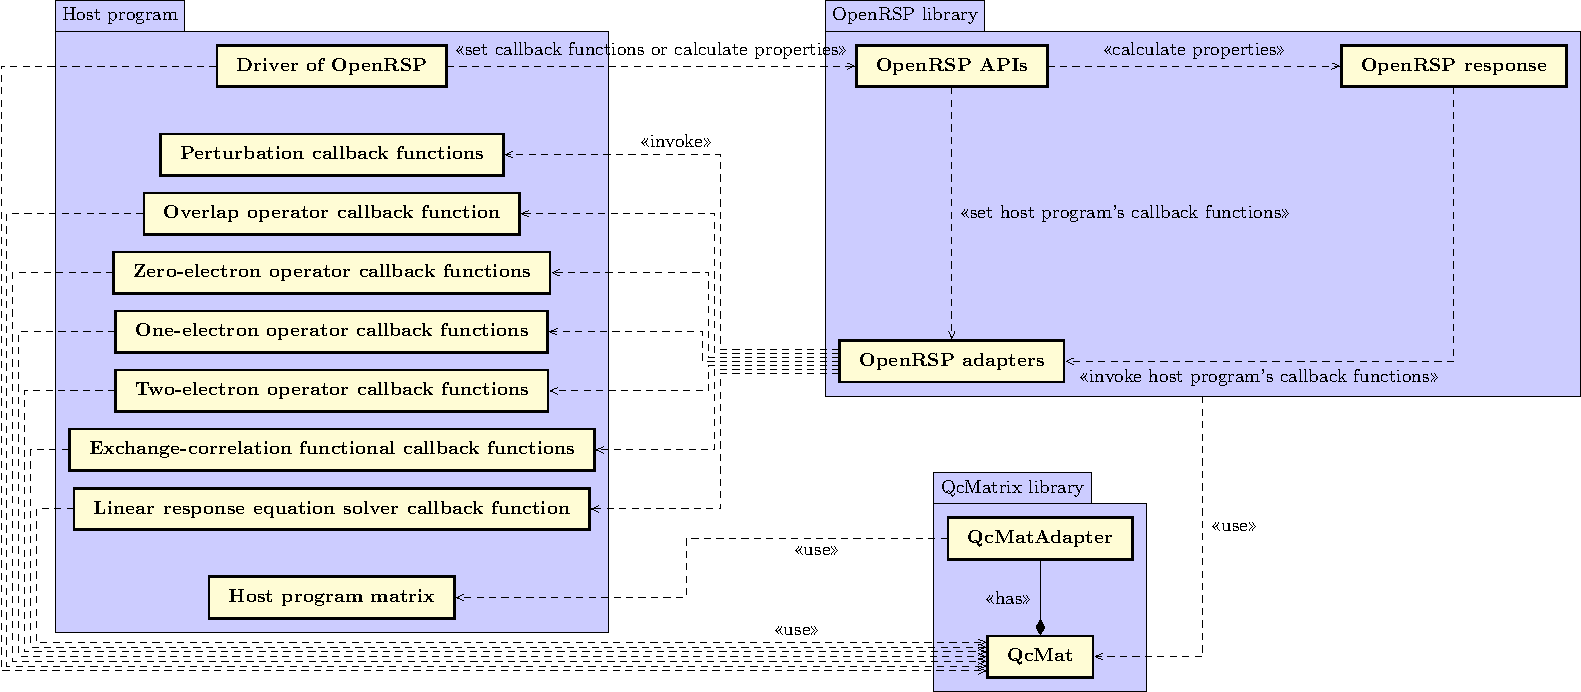
\includegraphics[width=0.45\textwidth]{openrsp_design.pdf}
  \caption{An overview of the software design of OpenRSP library.}
  \label{fig-openrsp-design}
\end{figure}

To make OpenRSP library open-ended, we need to make use of existing host
programs' source codes for the treatment of external perturbations, the
computation of Hamiltonian~(including both integral and expectation value
evaluations), the solving of linear response equations, as well as standard
matrix operations. Therefore, the challenge of developing such an open-ended
library is how to make it modular and portable so that it can be used in
different environments of host programs.

As shown in Fig.~\ref{fig-openrsp-design}, we have introduced the adapter
pattern in software engineering to achieve the best portability of OpenRSP
library. An adapter is also known as a wrapper that works as an extra layer
between the ``OpenRSP response'' part and host programs, so that only trivial
or no modifications are needed on the side of host programs.  Currently there
are 7 adapters implemented in OpenRSP library, for the ``OpenRSP response''
part to get information from host prgorams through the scheme of callback
functions, including information of perturbations, contributions from the
overlap operator, different one- and two-electron operators,
exchange--correlation~(XC) functionals and zero-electron operators~(which do
not depend on the knowledge of density matrix), as well as response parameters
solved from host programs' linear response equation solver.

Except for the adapters of perturbations and the linear response equation
solver, those of the overlap operator and various operators in the Hamiltonian
are not mandatory for OpenRSP library. For example, no XC functional adapter is
required to set for a Hartree-Fock calculation. Therefore, what kinds of
molecular response properties can be calculated are open-ended and are
completely decided by host programs---depending on what source codes existed in
host programs for the evaluations of operators in the Hamiltonian.

Last but not least, to also make use of host programs' matrix operations, we
have developed another stand-alone library QcMatrix (Version 0.1.0,
https://gitlab.com/bingao/qcmatrix), which can work as an adapter by (i) making
use of host programs' matrix operations and (ii) providing appropriate complex
matrix operations to OpenRSP library.

\subsubsection{Algorithms for the recursive evaluation of molecular response properties}
\label{subsubsection-recursive-algorithms}

% Something about the two major stages of the calculation: Perturbed F, D, S and assembling the property
From the various definitions of the terms that appear on the right-hand side of
Eq.~\eqref{master}, it can be seen that these terms contain perturbed and
unperturbed Fock, density and overlap matrices in addition to perturbed one-
and two-electron integral matrices, and, additionally, exchange--correlation
contributions in the cases where calculation at the DFT level is sought. As can
also be seen, apart from the perturbed $\mathbf{S}$ entering as the first
factor of the terms contained in $(\mathbf{SW})_{n_{W}}^{abc\cdots}$, the
maximum necessary order of perturbation to consider for the matrices
$\mathbf{F}$, $\mathbf{D}$, and $\mathbf{S}$ is dictated by the choice of
calculation rule $(k, n)$. As these matrices --- either perturbed or
unperturbed --- are used in several places in Eq.~\eqref{master}, a reasonable
approach is to calculate and store them before Eq.~\eqref{master} is evaluated
and then to apply them as needed for this purpose. Such storage can be
straightforwardly implemented by the use of linked lists where each list
element contains a header section describing a particular perturbation tuple
$b_{N}$ and a data section containing e.g. the matrices $\mathbf{F}^{b_{N}}$
perturbed with respect to the components of that perturbation tuple (and
likewise for the matrices $\mathbf{D}$ and $\mathbf{S}$). Moreover, if it is
known that several response properties are to be calculated, it is possible to
make use of the fact that the resulting terms on the right-hand side of
Eq.~\eqref{master} may contain one or more perturbed $\mathbf{F}$,
$\mathbf{D}$, and $\mathbf{S}$ that are common between more than one of the
properties. It can therefore be useful to have the linked lists be constructed
by identifying all necessary perturbed $\mathbf{F}$, $\mathbf{D}$, and
$\mathbf{S}$ for all properties for which calculation is desired, making new
entries only when a particular perturbation tuple was not encountered before.
The resulting list would therefore contain all desired perturbed matrices for
all properties while at the same time avoiding recalculation of common results.

A procedure to identify the needed perturbed $\mathbf{F}$, $\mathbf{D}$, and
$\mathbf{S}$ for a given choice of $(k, n)$ is described in Algorithm
\ref{ID-FDS} \fixme{MaR: Update the algorithm to encompass all of this and to
use the ``recurse --- then calculate'' approach and any new functionality since
the below version - such as identifying over several properties/freq. configs.}

\begin{algorithm}
\caption{Identify perturbed F, D, S ($b_{N}$)}
\label{ID-FDS}
\begin{algorithmic}
   \State {\it perturbation tuple}: $b_{N}$, $b_{N}^{*}$\\

   \If{$N > 1$}
      \For{$i$ in 1, $N$}
          \If{not already calculated} % VERIFY THIS SIMPLIFICATION
            \State $b_{N}^{*} \gets b_{N}$
            \State Remove $b_{N, i}^{*}$ from $b_{N}^{*}$
            \State call self($b_{N}^{*}$)
          \EndIf
      \EndFor
   % The else: was removed (VERIFY)
   \EndIf
   \If{not already calculated}
      \If{not truncating because of $(k,n)$ rule}
        \State call calculate perturbed F, D, S ($b_{N}$)
      \EndIf
   \EndIf
\end{algorithmic}
\end{algorithm}

In the traversal stage of Algorithm \ref{ID-FDS}, we note that the grouping of
the perturbed matrices is done in an order-by-order fashion since the
calculation of the perturbed $\mathbf{F}^{b_{N}}$ and $\mathbf{D}^{b_{N}}$ for
some perturbation tuple $b_{N}$ depends on the corresponding perturbed
$\mathbf{F}$ and $\mathbf{D}$ for all subsets of $b_{N}$. By proceeding order
by order, one can then assure that all required lower-order terms will be
available when needed. Applying the theory presented in
Section~\ref{rsp_theory}, and assuming that all such lower-order contributions
have already been obtained, Algorithm \ref{CALC-FDS} can be used to calculate a
given $\mathbf{F}^{b_{N}}$ and $\mathbf{D}^{b_{N}}$ (and $\mathbf{S}^{b_{N}}$).

\fixme{MaR: Update the algorithm to encompass all of this and to use the ``recurse --- then calculate'' approach and any new functionality since the below version}

\begin{algorithm}
\caption{Calculate perturbed F, D, S ($b_{N}$)}
\label{CALC-FDS}
\begin{algorithmic}
\State {\it perturbation tuple}: $b_{N}$, $b_{N}^{*}$\\

\State Get $\bm{\mathcal{S}}^{b_N}$
\State Construct $\breve{\bm{\mathcal{F}}}^{b_N}$ except terms involving $\mathbf{D}_{P}^{b_N}$ (VERIFY)
\For{component $i$ of $b_{N}$}
\State  $\mathbf{D}_{P, i}^{b_N} \gets \mathbf{Z}^{b_N}$ taking $\mathbf{D}_{i}^{b_N} = \mathbf{0}$ in the evaluation of $\mathbf{Z}^{b_N}$
\State  $\mathbf{D}_{P, i}^{b_N} \gets \mathbf{D}_{P, i}^{b_N} - \mathbf{D} \mathbf{S} \mathbf{D}_{P, i}^{b_N} - \mathbf{D}_{P, i}^{b_N} \mathbf{S} \mathbf{D}$ (VERIFY SIGNS)
 \State $\breve{\bm{\mathcal{F}}}_{i}^{b_N} \gets \breve{\bm{\mathcal{F}}}_{i}^{b_N} + \mathbf{G}^{KS}(\mathbf{D}^{b_N}_{P, i})$ (VERIFY RHS)
\State  Calculate $\mathbf{M}_{RHS}^{b_N}$ from eqn. \eqref{MRHS}
\State  Solve eqn. \eqref{LRE} (VERIFY) for $\mathbf{X}^{b_N}$ (-2 FACTOR?)
\State  $\mathbf{D}_{H, i}^{b_N} \gets \mathbf{X}^{b_N} \mathbf{S} \mathbf{D} - \mathbf{D} \mathbf{S} \mathbf{X}^{b_N}$
\State  $\breve{\bm{\mathcal{F}}}_{i}^{b_N} \gets \breve{\bm{\mathcal{F}}}_{i}^{b_N} + \mathbf{G}^{KS}(\mathbf{D}^{b_N}_{H, i})$ (VERIFY RHS)
\State  $\mathbf{D}_{i}^{b_N} \gets \mathbf{D}_{P, i}^{b_N} + \mathbf{D}_{H, i}^{b_N}$
\EndFor
\end{algorithmic}
\end{algorithm}

The identification of contributions to $\breve{\bm{\mathcal{F}}}^{b_N}$ in
Algorithm \ref{CALC-FDS} may be accomplished by the use of the recursive
Algorithm \ref{ID-CALC-FOCK}. The overall structure of this algorithm may also
be applied for the identification of contributing terms and subsequent
evaluation of $\mathcal{E}_{k,n}^{abc\cdots}$ of Eq.~\eqref{master}

\fixme{MaR: Update the algorithm to encompass all of this and to use the ``recurse --- then calculate'' approach and any new functionality since the below version}

\begin{algorithm}
\caption{Identify energy/Fock matrix contributions ($b_{N}$, $b_{\text{diff}}$)}
\label{ID-CALC-FOCK}
\begin{algorithmic}
\State {\it perturbation tuple}: $b_{N}$, $b_{N}^{*}$
\State {\it perturbation tuple, array(rank $=$ 1)}: $b_{\text{diff}}$, $b_{\text{diff}}^{*}$\\

   \If{$N > 0$}
      \For{$i$ in 1, length($b_{\text{diff}}$) + 1}
         \State $b_{\text{diff}}^{*} \gets b_{\text{diff}}$
         \If{$i =$ length($b_{\text{diff}}$)$ + 1$}
            \State Extend $b_{\text{diff}}^{*}$ by one tuple
            \State $b_{\text{diff}, i}^{*} \gets b_{N}$
         \Else
            \State Add $b_{N, 1}$ to $b_{\text{diff}, i}^{*}$
         \EndIf

         \State $b_{N}^{*} \gets b_{N}$
         \State Remove $b_{N, 1}^{*}$ from $b_{N}^{*}$
         \State Call self($b_{N}^{*}$, $b_{\text{diff}}^{*}$)
      \EndFor
   \Else

      \If{not already calculated}
         \If{not truncating because of $(k,n)$ rule}
            \If{considering lower-order Fock contributions}
               \If{$b_{\text{diff}, 2} \neq b_{N}$ of the initial (very first) call}
                  \State Calculate Fock contribution for $b_{\text{diff}}$
               \EndIf
            \ElsIf{considering energy-type contributions}
               \State Calculate energy-type contribution for $b_{\text{diff}}$
            \EndIf
         \EndIf
      \EndIf
   \EndIf
\end{algorithmic}
\end{algorithm}

A similar recursive product-rule algorithm can be constructed for the
identification of terms resulting from the differentiation of the four last
terms on the right-hand side of Eq.~\eqref{master} and is shown in
Algorithm~\ref{GET-DS}. These terms contain the matrices $\mathbf{W}$,
$\mathbf{\lambda}$, $\mathbf{Y}$, $\mathbf{\zeta}$, and $\mathbf{Z}$ (in
addition to the matrix $\mathbf{S}$ to be contracted with $\mathbf{W}$), which
are in turn mainly composed of products of three perturbed or unperturbed
$\mathbf{F}$, $\mathbf{D}$ or $\mathbf{S}$ matrices, as may be seen from their
definition, and Algorithm~\ref{GET-DS} may be used to identify these
three-matrix products in routines for the construction of the perturbed
$\mathbf{W}$, $\mathbf{\lambda}$, $\mathbf{Y}$, $\mathbf{\zeta}$, and
$\mathbf{Z}$, and may also be used to identify the various bra- and ket-side
differentiation combinations for perturbed matrices $\mathbf{T}$.

\fixme{MaR: Update the algorithm to encompass all of this and to use the ``recurse --- then calculate'' approach and any new functionality since the below version}

\begin{algorithm}
\caption{Get derivative superstructure (multiplicity $n$) ($b_{N}$, $b_{\text{diff}}$, $b_{\text{list}}$)}
\label{GET-DS}
\begin{algorithmic}
\State {\it perturbation tuple}: $b_{N}$, $b_{N}^{*}$
\State {\it perturbation tuple, dimension($n$)}: $b_{\text{diff}}$, $b_{\text{diff}}^{*}$
\State {\it perturbation tuple, dimension($n$), list}: $b_{\text{list}}$\\

   \If{$N > 0$}
      \For{i in 1, $N$}
         \State $b_{\text{diff}}^{*} \gets b_{\text{diff}}$
         \State Add $b_{N, 1}$ to $b_{\text{diff}, i}^{*}$
         \State $b_{N}^{*} \gets b_{N}$
         \State Remove $b_{N, 1}^{*}$ from $b_{N}^{*}$
         \State Call self($b_{N}^{*}$, $b_{\text{diff}}^{*}$, $b_{\text{list}}$) % MAYBE EVEN KN CHECK BEFORE RECURSING?
      \EndFor
   \Else
      \If{not truncating because of $(k,n)$ rule}
         \If{not truncating because of prime}
            \State Add $b_{\text{diff}}$ to $b_{\text{list}}$
         \EndIf
      \EndIf
   \EndIf
\end{algorithmic}
\end{algorithm}

Having shown how the various contributions in response property calculations
may be identified, we now turn to the actual evaluation of these contributions.

% Show use and utility of callback functionality, matrix operation mediation
% Show grouping together of terms
\section{\label{sec:VPT}Energy derivatives from variational perturbation theory}

\subsection{\label{sec:PDBS}Perturbation-dependent basis sets}

\section{\label{sec:QE-derivatives}Quasi-energy derivatives for self-consistent field wave functions}

\subsection{\label{sec:integrals}Evaluation of atomic integrals}

\subsection{\label{sec:XCkernels}Evaluation of exchange--correlation kernels}

\section{label{sec:conclusion}Concluding remarks}


\subsection{\label{sec:citeref}Citations and References}
A citation in text uses the command \verb+\cite{#1}+ or \verb+\onlinecite{#1}+
and refers to an entry in the bibliography. An entry in the bibliography is a
reference to another document.

\subsubsection{Citations}
Because REV\TeX\ uses the \verb+natbib+ package of Patrick Daly,
the entire repertoire of commands in that package are available for your document;
see the \verb+natbib+ documentation for further details. Please note that
REV\TeX\ requires version 8.31a or later of \verb+natbib+.

\paragraph{Syntax}
The argument of \verb+\cite+ may be a single \emph{key},
or may consist of a comma-separated list of keys.
The citation \emph{key} may contain
letters, numbers, the dash (-) character, or the period (.) character.
New with natbib 8.3 is an extension to the syntax that allows for
a star (*) form and two optional arguments on the citation key itself.
The syntax of the \verb+\cite+ command is thus (informally stated)
\begin{quotation}\flushleft\leftskip1em
\verb+\cite+ \verb+{+ \emph{key} \verb+}+, or\\
\verb+\cite+ \verb+{+ \emph{optarg+key} \verb+}+, or\\
\verb+\cite+ \verb+{+ \emph{optarg+key} \verb+,+ \emph{optarg+key}\ldots \verb+}+,
\end{quotation}\noindent
where \emph{optarg+key} signifies
\begin{quotation}\flushleft\leftskip1em
\emph{key}, or\\
\texttt{*}\emph{key}, or\\
\texttt{[}\emph{pre}\texttt{]}\emph{key}, or\\
\texttt{[}\emph{pre}\texttt{]}\texttt{[}\emph{post}\texttt{]}\emph{key}, or even\\
\texttt{*}\texttt{[}\emph{pre}\texttt{]}\texttt{[}\emph{post}\texttt{]}\emph{key}.
\end{quotation}\noindent
where \emph{pre} and \emph{post} is whatever text you wish to place
at the beginning and end, respectively, of the bibliographic reference
(see Ref.~[\onlinecite{witten2001}] and the two under Ref.~[\onlinecite{feyn54}]).
(Keep in mind that no automatic space or punctuation is applied.)
It is highly recommended that you put the entire \emph{pre} or \emph{post} portion
within its own set of braces, for example:
\verb+\cite+ \verb+{+ \texttt{[} \verb+{+\emph{text}\verb+}+\texttt{]}\emph{key}\verb+}+.
The extra set of braces will keep \LaTeX\ out of trouble if your \emph{text} contains the comma (,) character.

The star (*) modifier to the \emph{key} signifies that the reference is to be
merged with the previous reference into a single bibliographic entry,
a common idiom in APS and AIP articles (see below, Ref.~[\onlinecite{epr}]).
When references are merged in this way, they are separated by a semicolon instead of
the period (full stop) that would otherwise appear.

\paragraph{Eliding repeated information}
When a reference is merged, some of its fields may be elided: for example,
when the author matches that of the previous reference, it is omitted.
If both author and journal match, both are omitted.
If the journal matches, but the author does not, the journal is replaced by \emph{ibid.},
as exemplified by Ref.~[\onlinecite{epr}].
These rules embody common editorial practice in APS and AIP journals and will only
be in effect if the markup features of the APS and AIP Bib\TeX\ styles is employed.

\paragraph{The options of the cite command itself}
Please note that optional arguments to the \emph{key} change the reference in the bibliography,
not the citation in the body of the document.
For the latter, use the optional arguments of the \verb+\cite+ command itself:
\verb+\cite+ \texttt{*}\allowbreak
\texttt{[}\emph{pre-cite}\texttt{]}\allowbreak
\texttt{[}\emph{post-cite}\texttt{]}\allowbreak
\verb+{+\emph{key-list}\verb+}+.

\end{document}
%
% ****** End of file apssamp.tex ******
